\section{How it works}
This section describes how self-propelled instrumentation works in details.
Each subsection is a major step in the workflow.

% The workflow:
% 1. injector hijacks a process
% 2. agent is loaded in the process
% 3. init function in agent is executed
% 3.1 register event
% 3.2 register payload function
% 3.3 other configuration
% 4. event activation, doing initial instrumentation
% 5. propagation



\subsection{Building Agent}
Users build their own {\em Agent} shared library using self-propelled
instrumentation's API.
\begin{enumerate}
\item Coding. Users need to write two pieces of code: 1) payload function; 2)
  configuration code that registers payload function and does some
  customization
  and configuration. The configuration code must be executed right away
  when the
  {\em Agent} shared library is loaded into the application process, so the
  configuration code should be in the init function of the {\em Agent} shared
  library, i.e., the function with gcc directive
  \_\_attribute\_\_((constructor)).
\item Building. Users build the code into an {\em Agent} shared library linking
  with {\em libagent.so} provided by the self-propelled instrumentation
  infrastructure.
\end{enumerate}

\subsection{Injection}
Users run {\em Injector} in command line. They specify in command line
arguments
the path of an {\em Agent} shared library and the application process to inject
to.

One trick to check whether the {\em Agent} shared library is injected
successfully is to look at memory maps file of the application process, i.e.,
/proc/PID/maps.

\subsection{Initialisation} %changed configuration to initialisation as
per diagram
The initialisation code is executed right away when {\em Agent} shared
library is
loaded into the application process.
It tells self-propelled instrumentation what are payload functions provided by
users, how would initial instrumentation be done, whether or not to enable
inter-process instrumentation propagation ...

\subsection{Initial Instrumentation}
Once the configuration code in the {\em Agent shared library} finishes
execution
inside the application process, the initial instrumentation would be performed
right away, e.g., instrumenting all function calls inside the {\em main}
function.

\subsection{Instrumentation Propagation}
When one of the initial instrumentation gets executed, then instrumentation
propagates itself either within the process by following control flow,
or across
process boundaries by following communication flow.

% May put intra-process propagation and inter-process propagation diagram here
\subsubsection{Intra-process propagation}
\begin{figure}[ht]
  \centering
  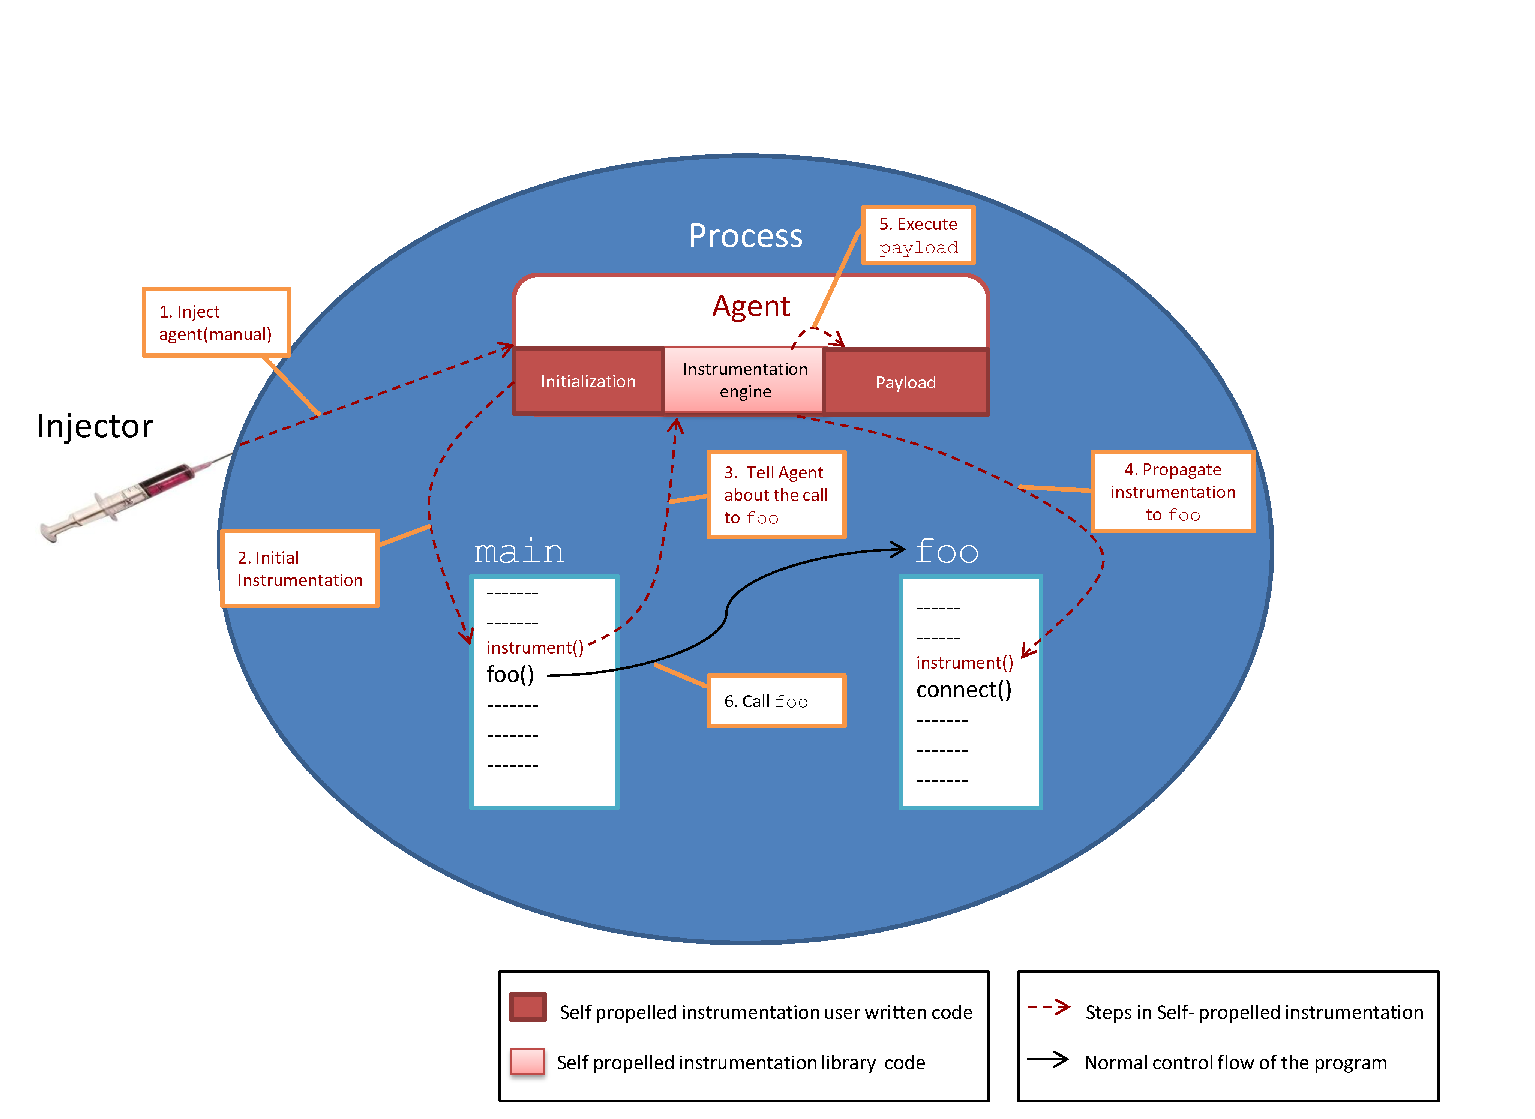
\includegraphics[width=0.90\textwidth]{figure/intraprocess.eps}
  \caption{Intra-process Self-propelled Instrumentation Workflow}
   \label{fig:Intra-process Self-propelled Instrumentation}
\end{figure}

Instrumenting all the function calls inside {\em main} function
internally calls the instrumentation engine, before each function
call. Instrumentation engine, in turn, propagates the instrumentation to
the called
function. If the called
function is within the same process, then instrumentation engine directly
propagates the instrumentation to the called function: i.e it instruments
all the function calls inside the called
function.  The instrumentation engine
also executes payload function either before instrumenting or after
instrumenting depending
on whether it is an entry payload or exit payload function. After the
instrumentation is done, the application's normal intra-process function
call execution
takes place. The workflow is visualized in Figure~\ref{fig:Intra-process
Self-propelled Instrumentation}.


\subsubsection{Inter-process propagation}
\begin{figure}[ht]
  \centering
  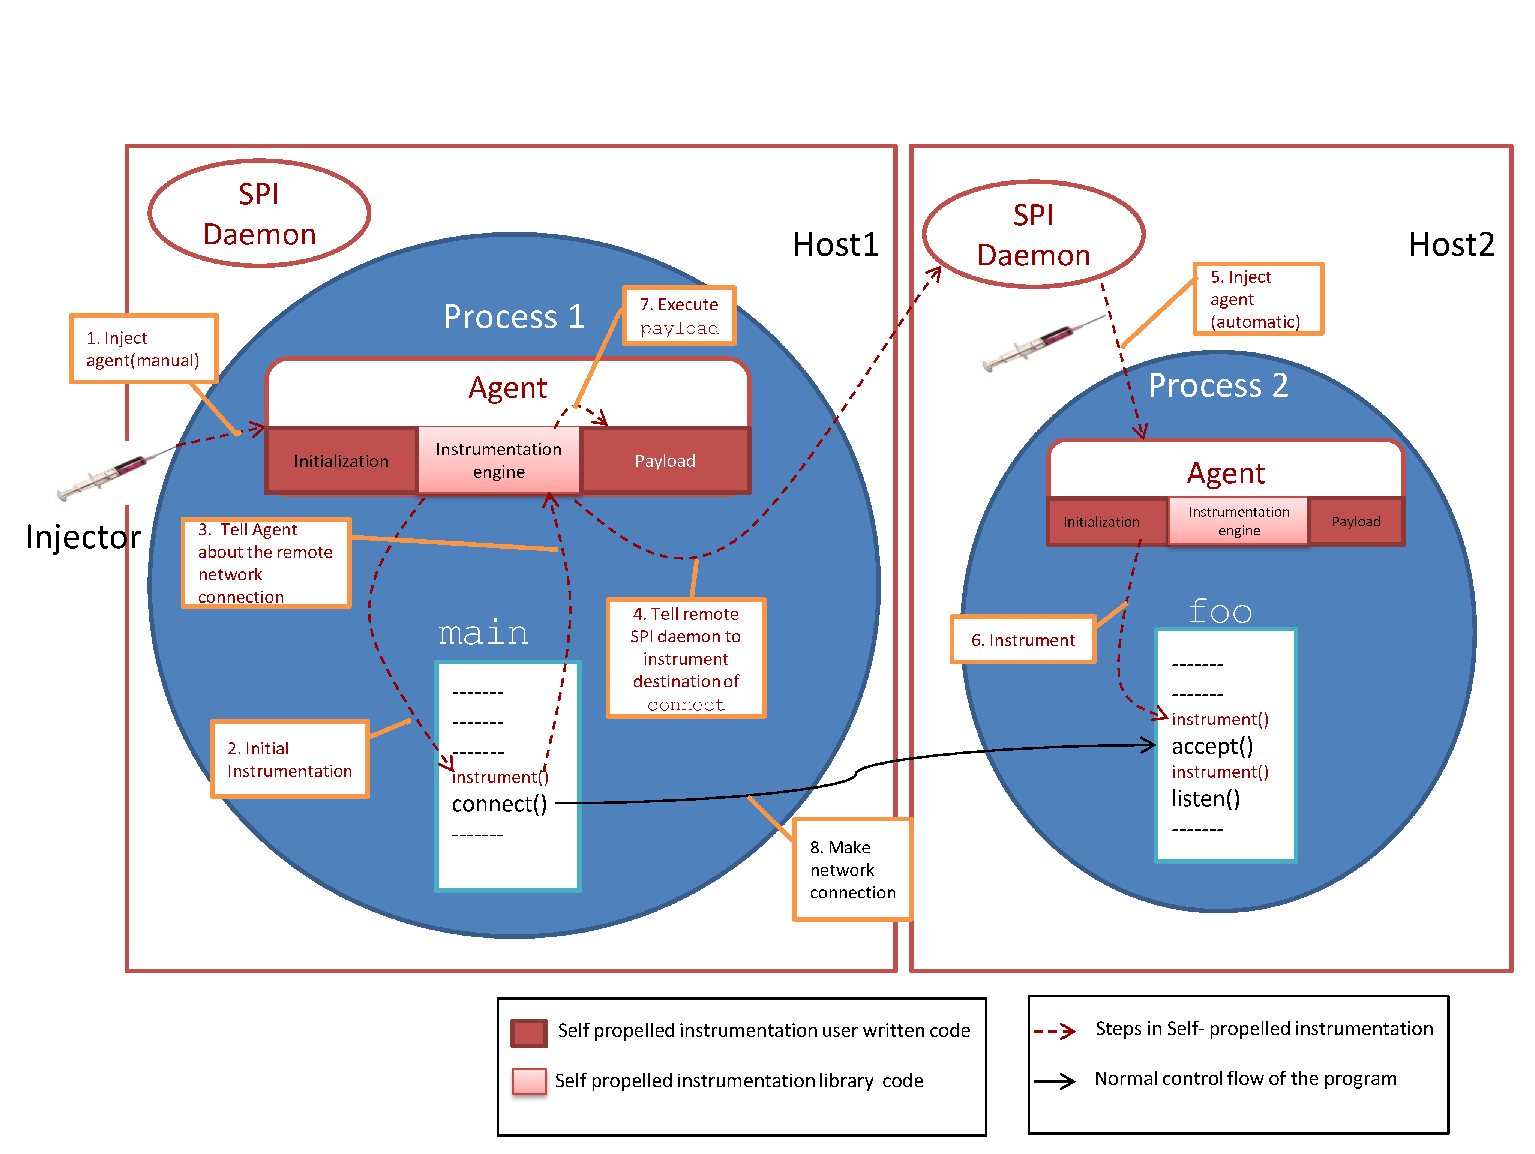
\includegraphics[width=0.90\textwidth]{figure/interprocess.eps}
  \caption{Inter-process Self-propelled Instrumentation Workflow}
  \label{fig:Inter-process Self-propelled Instrumentation}
\end{figure}

Similar to intra-process propagation, inter-process propagation also
instruments all the function calls inside an instrumenting function, with
the difference that
called function lies in a different process or host. So the instrumentation
engine, which gets called before every function call of the instrumenting
function, identifies that the called function is an inter-process function. It
then propagates the call to the SPI daemon of the appropriate host where
the called function is present.
The called SPI daemon then injects the agent shared library automatically
inside the process where the called function is located. Then the usual
process of \textit{initialisation} and \textit{initial instrumentation} goes
on inside the called function. After the instrumentation is done, the
application's normal inter-process function call execution takes place. In
the mean time, the instrumentation engine executes the payload depending on
whether it is an entry payload or an exit payload. The workflow is visualized
in Figure~\ref{fig:Inter-process Self-propelled Instrumentation}.




